\section{Magnetisches Feld}
\subsection{Moodle-Übung}
\begin{enumerate}
  \item Magnetische Kraft zwischen zwei parallel verlaufenden, stromdurchflossenen geraden Leitern wobei $a >> d$
        \begin{figure}[h!]
          \begin{center}
            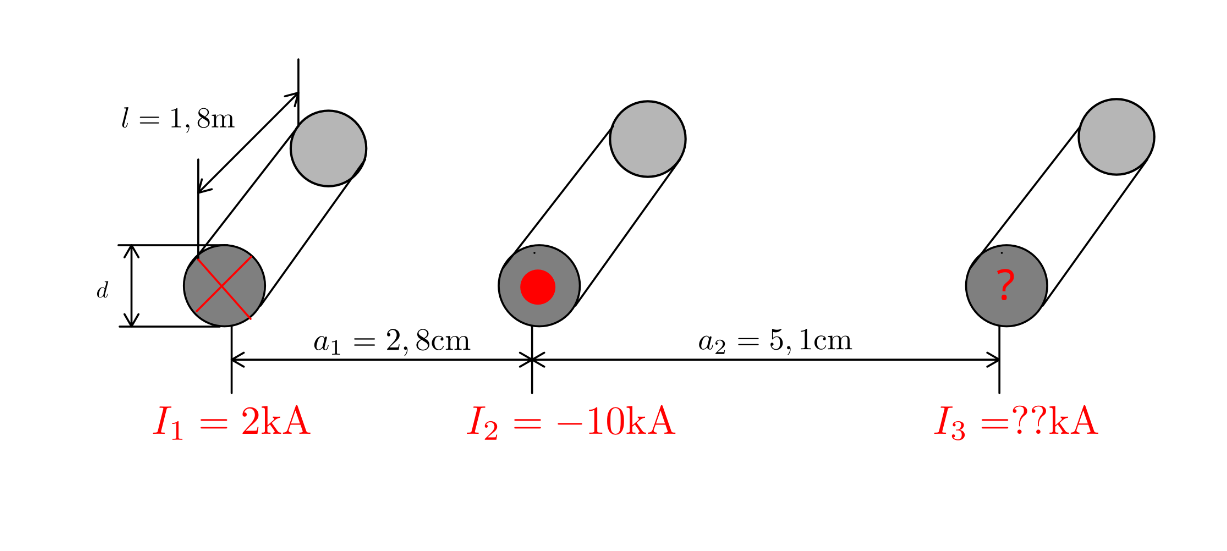
\includegraphics[width=0.75\textwidth]{img/Magnetisches-Feld/A1.png}
          \end{center}
          \caption{Moodle-Übung magnetisches Feld – Kraftwirkung auf drei Leitern}
        \end{figure}

        \begin{align*}
          F_{12}             & = \frac{\mu}{2\pi}\cdot \frac{I_1\cdot I_2}{a}\cdot l                                 \\
          \text{Für } F_{12} & = F_{32} \text{ dann gilt:}                                                           \\
          I_3                & = \frac{I_1\cdot a_2}{a1}                                                             \\
                             & = \frac{2\cdot 10^{3}\text{A}\cdot 5,1\cdot 10^{-2}\text{m}}{2,8\cdot 10^{3}\text{m}} \\
                             & = 3,64\text{kA}                                                                       \\                                                                   \\
        \end{align*}

        \begin{align*}
          F_{31} & =\frac{\mu\cdot\mu_{0}}{2\pi}\cdot\frac{I_{1}\cdot I_{3}}{a}\cdot l                                                                                                                        \\
                 & =\frac{4\pi\cdot 10^{-7}\frac{\text{H}}{\text{m}}}{2\pi}\cdot\frac{2\cdot 10^{3}\text{A}\cdot 3,64\cdot 10^{3}\text{A}}{2,8\cdot 10^{-2}\text{m}+5,1\cdot 10^{-2}\text{m}}\cdot 1,8\text{m} \\
                 & =-33,202\text{N}                                                                                                                                                                           \\
                 & \Rightarrow |33,20\text{N}|                                                                                                                                                                \\                                                                                                                                                                 \\
        \end{align*}

        \begin{align*}
          F_{21} & =\frac{\mu\cdot\mu_{0}}{2\pi}\cdot\frac{I_{2}\cdot I_{1}}{a}\cdot l                                                                                                                         \\
                 & =\frac{4\pi\cdot 10^{-7}\frac{\text{H}}{\text{m}}}{2\pi}\cdot\frac{2\cdot 10^{3}\text{A}\cdot(-10\cdot 10^{-2}\text{A})}{2,8\cdot 10^{3}\text{m}+5,1\cdot 10^{-2}\text{m}}\cdot 1,8\text{m} \\
                 & =-33,202\text{N}                                                                                                                                                                            \\
                 & \Rightarrow |33,20\text{N}|                                                                                                                                                                 \\                                                                                                                                                              \\
        \end{align*}

\end{enumerate}
